 \documentclass[conference]{IEEEtran}
\IEEEoverridecommandlockouts
% The preceding line is only needed to identify funding in the first footnote. If that is unneeded, please comment it out.
\usepackage{cite}
\usepackage{amsmath,amssymb,amsfonts}
\usepackage{algorithmic}
\usepackage{graphicx}
\usepackage{float} 
\usepackage{subfigure} 
\usepackage{textcomp}
\usepackage{xcolor}
\def\BibTeX{{\rm B\kern-.05em{\sc i\kern-.025em b}\kern-.08em
    T\kern-.1667em\lower.7ex\hbox{E}\kern-.125emX}}
\begin{document}

\title{Implementation and Deployment: Tripedia\\
}

\author{\IEEEauthorblockN{Yulin Zhang}
\IEEEauthorblockA{\textit{7th Group} \\
\textit{Software Engineering}\\
Montreal, Canada \\
silveralex2023820@gmail.com}
\and
\IEEEauthorblockN{Yuhang Chen}
\IEEEauthorblockA{\textit{7th Group} \\
\textit{Software Engineering}\\
Montreal, Canada \\
yuhang.chen@mail.concordia.ca}
\and
\IEEEauthorblockN{Jiaxi Yang}
\IEEEauthorblockA{\textit{7th Group} \\
\textit{Software Engineering}\\
Montreal, Canada \\
yjxyang2@outlook.com}
\and
\IEEEauthorblockN{Boyang Wang}
\IEEEauthorblockA{\textit{7th Group} \\
\textit{Software Engineering}\\
Montreal, Canada \\
wangboyang0626@outlook.com}
}

\maketitle


\begin{figure*}[htbp]
\centerline{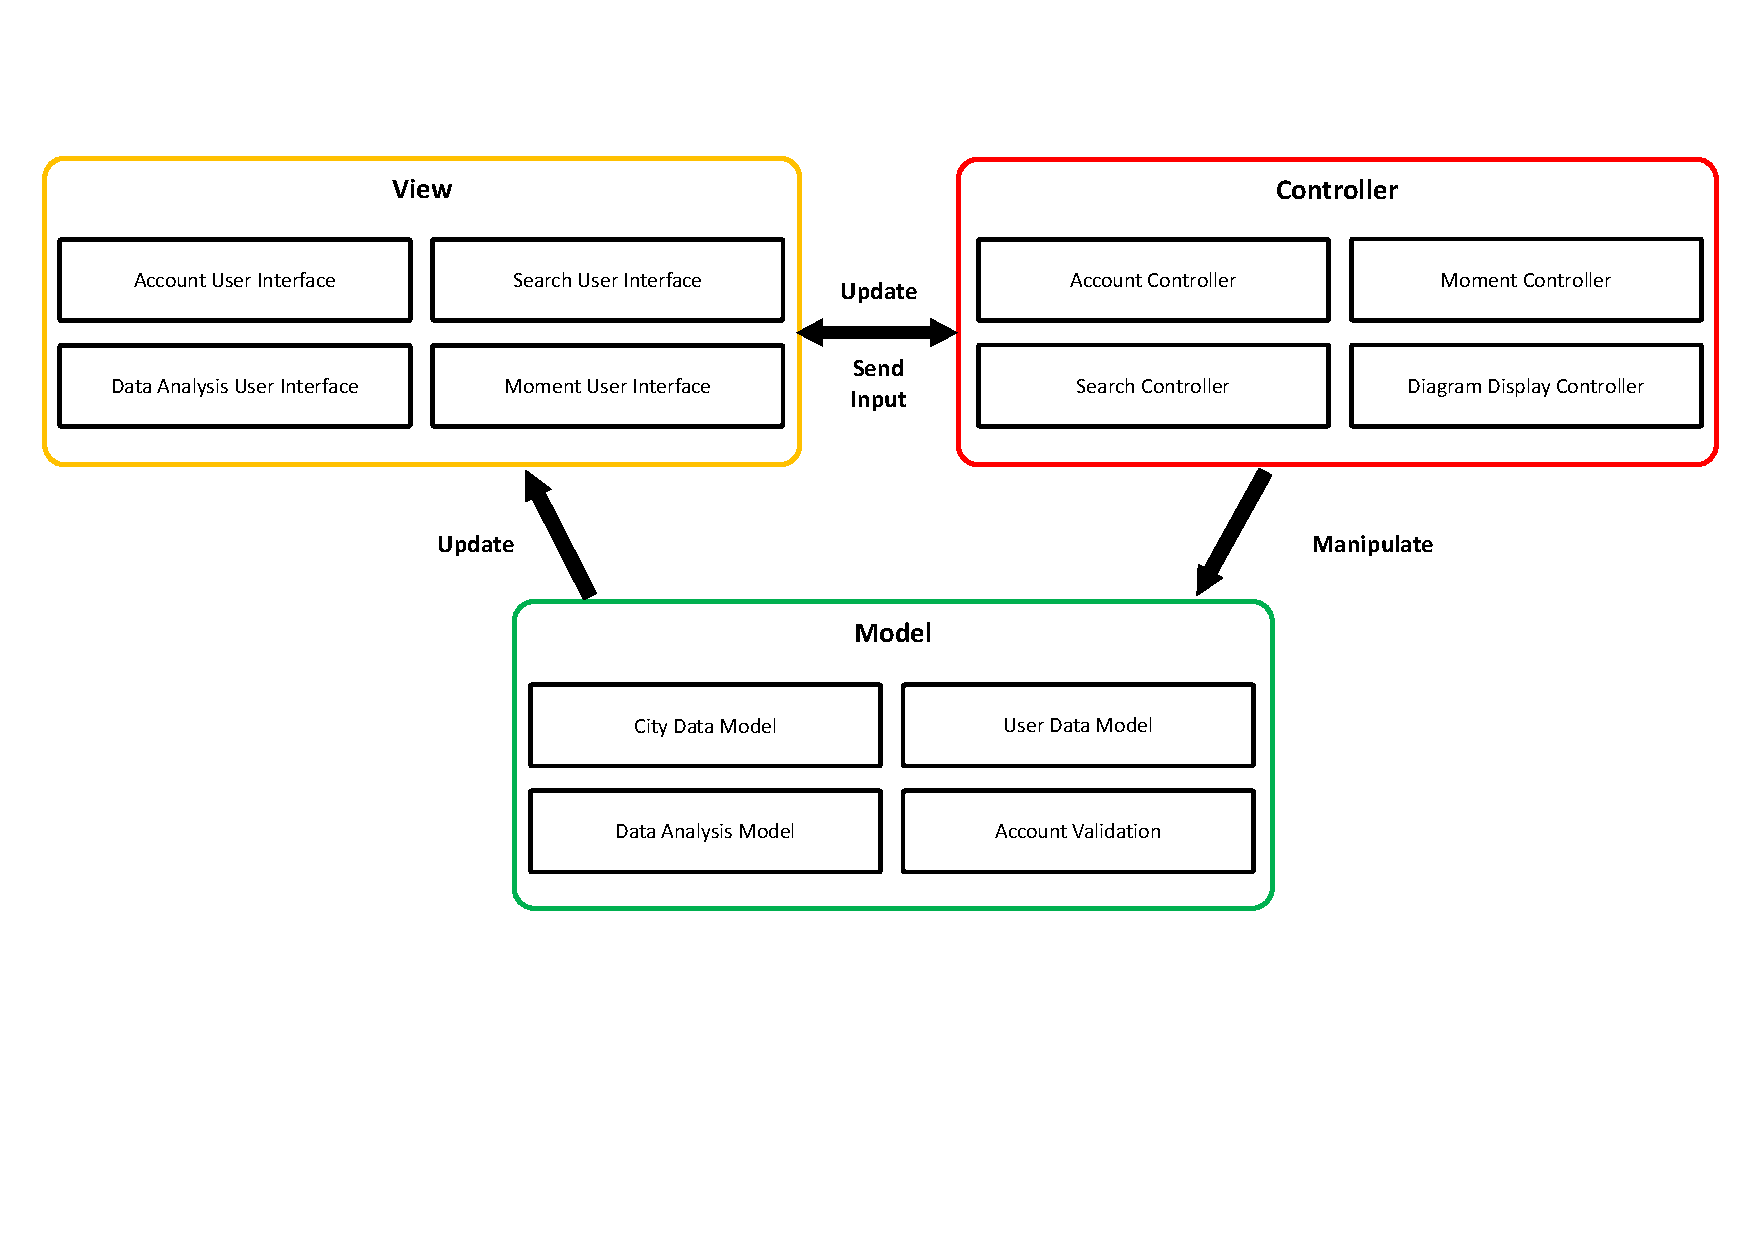
\includegraphics[width=1.0\textwidth]{Architecture.pdf}}
\caption{The Adoption of MVC Pattern in Tripedia.}
\label{system_mvc}
\end{figure*}





\section{\textbf{Architectural Design Process}}

\textbf{Question: Identify and articulate what are your architectural designs and the associated
software engineering process.}

Architectural designs serve as the blueprints for our software systems, shaping their form and defining the relationships among components. Our design choice comes with its own set of considerations and implications. In this chapter, we will dissect the architectural design of the Tripedia system. 


\subsection{\textbf{Architectural Design}}

In our system, we adopted the \textbf{MVC Architectural Pattern}. At the same time, we have referred to the design philosophy of \textbf{Layered Architectural Pattern}. We try our best to decouple the logic by architectural design and achieve great results.

The architectural design is shown in figure\ref{system_mvc}. Meanwhile, the detail is introduced in Chapter III: the adoption of MVC and Layered Architecture.


\subsection{\textbf{Software Engineering Process}}

Beginning in the Specification phase, our vision was to construct a dynamic and feature-rich tourist website. In this stage, we chose the MVC architecture as our application architecture. This structure is ideally suited to the website we envisioned containing multiple ways of viewing and interacting with data.

During the design phase, we looked to the MVC framework to help us choose the right technologies. After careful consideration, we opted for Flask, a technology renowned for its strong MVC support. This decision laid a solid foundation for the subsequent stages of development.

As we forged ahead into the development phase, we decided to adopt a decentralized control strategy that distributes control among components. For example, in the searching function, I created a lot of searching APIs, which can call different crawlers to get information from the internet. Each of these interfaces can operate independently of each other. which Greatly increases the stability and maintainability of the system.

Once we entered the Validation phase, our MVC architecture proved its worth. The isolation of the model, view, and controller components allowed us to perform targeted testing and debugging very effectively.



\section{\textbf{Architecture Design Consideration}}

\textbf{Question: Indicate if any revision to your architectural design is necessary. If the answer is Yes, please explain what revision, and the reason.}

In this chapter, we will explore the scenarios of our system. And we will give reasons for our decision about revision.

\subsection{\textbf{Revision Consideration}}

To be honest, we \textbf{did not do any revision} in our architectural design. 

\subsection{\textbf{Reasons}}

There are several reasons about why we did not change our architectural structure. 

(1) We have adequate initial planning in our project. At the beginning of the development, we have carefully designed the development framework and possible future development plans. This careful planning ensured that the architecture was well-suited to meet the project's requirements.

(2) Our architecture is flexibility and scalability. Our architecture is stable enough for us to expand functions. We did not meet any obstacles in our development. This adaptability helped in avoiding major architectural revisions.

(3) Our system has great technological compatibility. The selected technology stack and tools were fully compatible with the chosen architecture, ensuring smooth development and operation processes.

(4) Our project is a prototype, we have no need to concern the bussiness requirements. 



\section{\textbf{The Adoption of MVC and Layered Architecture}}

\textbf{Question: Further adopt MVC and Layered Architecture Pattern to your ICDE-App. Describe your design decisions, and discuss the pros and cons of the design.}

In this chapter, we discuss the adoption of MVC and Layered Architecture Patterns into the Tripedia system. By embracing these architectural patterns, we aim to achieve a balance between flexibility, scalability, and maintainability. Finally, we explain the pros and cons of our system architecture.


\subsection{\textbf{The Adoption of MVC Architecture Pattern}}

As shown in figure\ref{system_mvc}, our system mainly adopt the MVC Architecture Pattern. Our system can be divided into three parts: View, Controller and Model.

In the View part, we implement multiple user interfaces based on the web pages, which is responsible for data presentation and the interaction with users. For example, the Data Analysis User Interface provides the questionnaire to capture user's preference data, and presents the analysis results with html diagram.

The controller worked as the bridge between the View and the Mode. The controller gather the requests sent from the View and processes the request based on the Model services. For example, the diagram display controller gets the request of presenting the analysis result. The Diagram display controller manipulates the Data Analysis Model in Model part to gain the results. Finally, the results are returned to the View part by the Diagram Display Controller.

The model focuses on the data processing. For example, the data analysis model provide the interfaces of data analzing for the controller. 

Above all, our system adopted a standard MVC architecture in the development.

\begin{figure*}[htbp]
\centerline{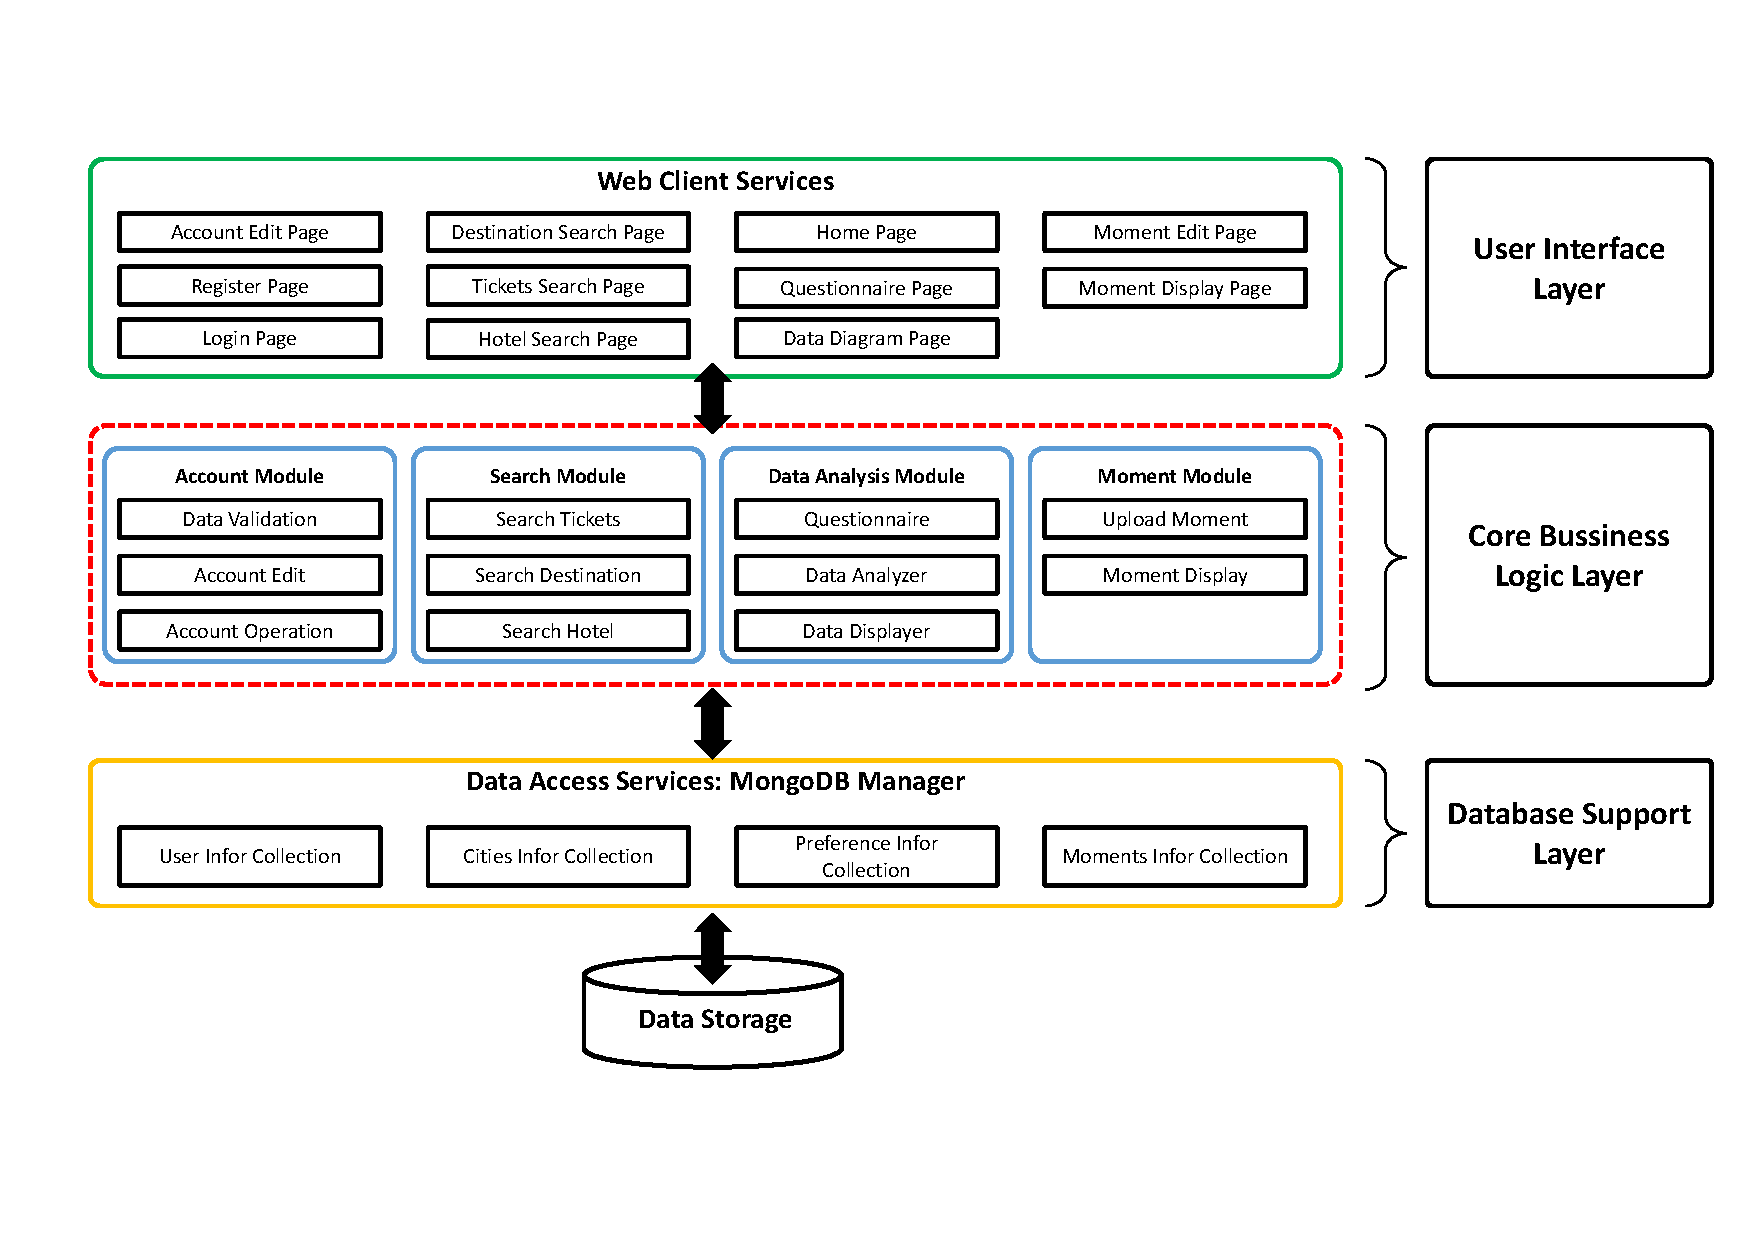
\includegraphics[width=1.0\textwidth]{Architecture2.pdf}}
\caption{The Adoption of Layered Architecture Pattern in Tripedia.}
\label{system_layered}
\end{figure*}


\subsection{\textbf{The Adoption of Layered Architecture Pattern}}

From layered architectural views, our system develops in a systematic way to organize and structure code. The layered architectural pattern divides the software application into distinct layers, each responsible for a specific set of functionalities. The layers are arranged hierarchically, with each layer interacting primarily with the layers immediately above and below it. 

As shown in figure\ref{system_layered}, our system is designed in three layers: 

\begin{itemize}
    \item User Interface Layer: responsible for interacting with users and presenting information in a user-friendly manner.

    \item Core Bussiness Logic Layer: responsible for implementing the core business rules, logic, and processes of the application.

    \item Database Support Layer: responsible for supporting mongodb unique interfaces.
\end{itemize}


In user interface layer, we focus on the designing and development of web pages. In this part,  There are multi modules in our system, and each system needs a user-friendly interface. These web pages are interact with the Core Bussiness Logic Layer. For example, when users wanna to login to our system, they will interact with the login page of User Interface Layer. Furthermore, the operation of users sends to the Core Bussiness Logic Layer, and the module in Core Bussiness Logic Layer response for the requests.

In Core Bussiness Logic Layer, we implement a series of server functions, which are the core functions of the system. The account module is responsible for the issues of account operations. The search module processes the search functions based on the crawling. The data analysis module provides a set of recommendation services based on user preference data. Finally, the moment module provides a platform for user to share their travel experience.

In Database Support Layer, we designed and implemented different database interface for different data structure. The Database Support Layer provides unique database interfaces to support the processing of the Core Bussiness Logic Layer.

Above all, we adopted the design philosophy of Layered Architecture into our system, which makes our development process more smooth.



\begin{table*}[htbp]
\caption{The software metrics and granularity of components.}
\begin{center}
\begin{tabular}{|c|c|c|c|}
\hline
\textbf{Task Name} & \textbf{\textit{LOC}}& \textbf{\textit{Component Granularity Level}}& \textbf{\textit{Numbers of Units}} \\
\hline
Data Displayer & 274  & packages & 1 \\
KNNDataAnalayzer & 106 & Python Class &  6 \\
Questionnaire & 169 & packages & 1 \\
MongoDBManager & 35 & Python Class & 2 \\
UserInfoCollection & 40 & Python Class & 2 \\
CitiesInfoCollection & 66 & Python Class & 2 \\
Seacher & 238 & packages & 4\\
HotelCollector & 161 & packages & 3\\
TicketCollector & 228 & packages & 3\\
DestinationCollector & 74 & packages & 2\\
Moments & 33 & Package & 1\\
Account Manager& 91 &packages&1\\

Flask & NA & Framework & 1 \\
MongoDB & NA & Framework & 1 \\

\hline
\end{tabular}
\label{tab1}
\end{center}
\end{table*}
\subsection{\textbf{The Pros and Cons}}

We try our best to combine the MVC and Layered Architecture patterns, which brings several advantages to our ICDE application. Meanwhile, the architecture also comes with potential drawbacks.

The advantages of our system architecture are as follows:

\begin{itemize}
    \item Maintainability: By breaking the application down into modular components, it becomes easier to pinpoint and address issues, increasing the application's maintainability.

    \item Scalability:  Both the MVC pattern and layered architecture pattern support building scalable applications. In our project, adding new features or modifying existing ones can be done without affecting other parts of the codebase.

    \item Testability: The separation provided by these patterns makes unit testing and integration testing more straightforward, enhancing the application's quality.

\end{itemize}

On the other hand, our system also has some shortcomings.

\begin{itemize}
    \item Performance Overhead: Because of the transmission of information, our architecture may introduce performance overhead.

    \item Complexity:  MVC and layered architecture patterns can introduce complexity to the application as you need to manage multiple components and their interactions.

\end{itemize}

In conclusion, applying MVC and layered architecture patterns to the ICDE application can enhance its maintainability, scalability, and testability but also requires a balance between complexity and performance considerations.


\section{\textbf{Software Metrics and Granularity of Components}}

\textbf{Question: Please make a statistical count of software metrics from all your tasks implemented so far and
form a table given the template below. }

Our development statistics is shown in table\ref{tab1}. 


\section{ \textbf{ Unitest Case in White-box Testing}}

The white-box testing in our project is to ensure the correctness of the internal logic, uncover any code-based errors, and verify the completeness of the codebase. On the other hand, white-box testing will also cover critical components of the codebase where precision and accuracy are paramount. Hence, we did some white-box tests based on the Data Analyzing Module.


\subsection{ \textbf{ Unitest Case: KNN Analyzer }}

KNN Analyzer is the most essential part in our ICDE system. The correctness of the data calculation is important.
The unitest case is implemented in the KNNDataAnalayzer\_test\_case() function.

 \textbf{ Input: }

1. The user name 'zhangyulin'.


 \textbf{ Tests: }

1. Create an instance of KNN Analyzer.

2. Find the preference data of 'zhangyulin', and further analyze the recommended cities data.

3. Print the recommended cities' names and recommend cities' scores.

 \textbf{ Output: }

1. The first line of the output should be as follows:

['Calgary', 'Halifax', 'Yukon', 'QuebecCity', 'Fredericton']

2. The second line of the output should be as follows:

[101.9, 118.9, 127.3, 128.4, 169.6]



\subsection{ \textbf{ Unitest Case: Introduction Generator }}

In the data display module, our system transferred the analyzed data in a visible format. In this part, we test the correctness of the calculation in function generate\_preference\_introduction\_test\_case() and generate\_popular\_introduce\_test\_case().

 \textbf{ Input: }

1. The user name 'zhangyulin'.


 \textbf{ Tests: }

1. Create an instance of KNN Analyzer.

2. Generate the auto introduction based on the preference data.

3. Generate the auto introduction based on the popular cities' data.

4. Print the recommended introduction and the popular cities' introduction.

 \textbf{ Output: }

1. The first line of the output should be as follows, which is the auto introduction to the recommended data.

Bonjour! According to the psychological testing, the best tourist destination for your is Calgary. Calgary has awsome natural environment (the natural rate is 97), you can release your workload and enjoy yourself. Calgary is also a famous historical city (the historical rate is 45), you can find a great number of interesting history stories here. Calgary is well-known because of her culture (the historical rate is 80), you can meet interesting people here. 


2. The second line of the output should be as follows:

In this season, the most popular city is Toronto. 


\subsection{ \textbf{ Unitest Case: Unique Database Interface }}


In the database interface module, our system provides a series of stable interfaces for the other modules. In this part, we test the correctness of the data access services in function city\_infor\_manager\_test\_case() and user\_preference\_test\_case().


 \textbf{ Input: }

1. The city name 'Calgary'.

2. The username 'zhangyulin'.

 \textbf{ Tests: }

1. Access the city's properties based on the city name 'Calgary'.

2. Access the preference data based on the user name 'zhangyulin'.

3. Print the accessed data.

 \textbf{ Output: }

1. The first part of the output is related to the city data, which is shown as follows:

city population: 1988

city metropolis: 34

city mountain: 1

city historical: 45

city humanistic: 80

city natural: 97


2. The second part of the output is related to the reference data, which is shown as follows:

user workload preference: 80

user history preference: 80

user nature preference: 100

user noisy preference: 20

user quite preference: 80

user sports preference: 1


\section{ \textbf{ Unitest Case in Black-box Testing}}


Black-box testing is a software testing method where the internal workings or logic of the system being tested are not known to the tester. Our primary objective of black-box testing in our project is to ensure that the software functions according to its specified requirements and meets the expectations of end-users. So, in this chapter, we discussed some black-box tests in our project.



\subsection{ \textbf{ Account Module Testing}}

\textbf{ Objective: }

Verify that the user account functionality in our system works as expected.

\textbf{Test Steps: }

Navigate to the Login Page:

(1) Navigate to the login page.

(2) Enter a valid username and password.

(3) Click the "Login" button.

(4) Verify Successful Login.

(5) Ensure that the user is redirected to the home page. Confirm that the user's name is displayed indicating a successful login.

Enter Invalid Credentials:

(1) Enter an invalid username or password.

(2) Click the "Login" button.

(3) Verify Error Message:

(4)Confirm that an appropriate error message is displayed. Ensure the user is not logged in with invalid credentials.

\textbf{Expected Results: }

For valid inputs, the user should be successfully logged in. For invalid inputs, an appropriate error message should be displayed, and the user should not be logged in.

\subsection{ \textbf{ Search Module Testing}}

\textbf{ Objective: }

Verify the correctness and efficiency of the search algorithm in our system.

\textbf{Test Steps: }

(1) Navigate to the Search Hotels page.

(2) Enter the target destination and the check-in/check-out dates.

(3) Click the "Search" button.

(4) Ensure that the hotels' information is the same as the results expected.

\textbf{Expected Results: }

The search algorithm should return accurate results based on the search query. Meanwhile, the search should be performed efficiently under different conditions.



\subsection{ \textbf{ Data Analyzer Testing}}

\textbf{ Objective: }

Verify the correctness and efficiency of the data analyzing algorithm in our system.

\textbf{Test Steps: }

(1) Navigate to the Questionnaire page.

(2) Enter the preference data according to the questions.

(3) Click the "Submit" button.

(4) Navigate to the Recommendation page.

(4) Ensure that the analyzed data is the same as the results expected.

\textbf{Expected Results: }

The analyzing algorithm should return accurate results based on the user's preference data. Meanwhile, the diagram and introduction should explain the results clearly and directly.











































\end{document}
